
\subsection{Basics}
The goal of MAC is to prevents tampering with a message. MAC require a secret
key otherwise modification of the message cannot be done. MAC ensures integrity,
authentication but not confidentiality.

\subsection{Constructions}
Let h be a hash function, k a key, m the message to be MACed, and M the
computed MAC\@.
\begin{itemize}
    \item Prefix method: $ M = h(k||m) $
    \item Suffix method: $ M = h(m||k) $
    \item Envelop method:$ M = h(k||p||m||k) $
\end{itemize}
MAC uses hash function rather than block cipher because hash function are
generally faster.
\begin{figure}[ht!]
    \centering
    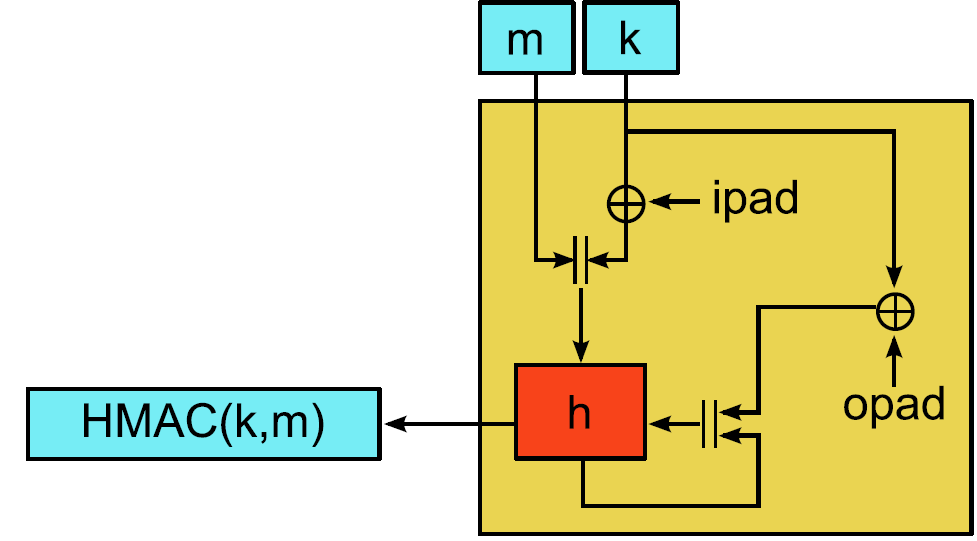
\includegraphics[scale=0.5]{img/hmac}
\end{figure}

\subsubsection{Built upon a cipher}
Based on the CBC mode of operation
\begin{itemize}
    \item The message is encrypted in CBC mode
    \item Final block is the MAC
    \item Intermediary blocks are thrown out
    \item IV consists of zeros
\end{itemize}

\begin{figure}[ht!]
    \centering
    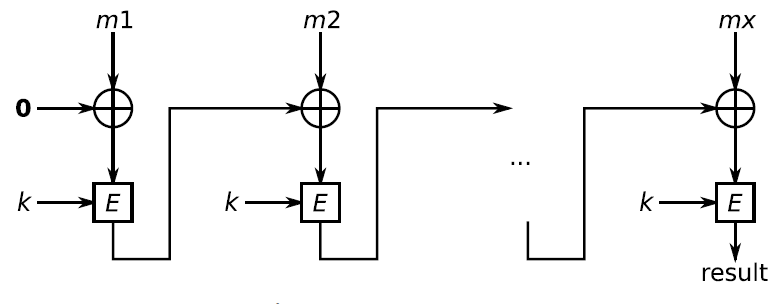
\includegraphics[scale=0.5]{img/cbc-mac}
\end{figure}

\begin{itemize}
    \item CBC-MAC is secure for messages of a fixed number of blocks assuming
    the block cipher is secure.
    \item Not secure with variable lengths
    \item CBC-MAC $(length(M)||M)$ to avoid truncation attacks
    \item Encrypt $length(M)$ with K, yielding K' and use it as key for the
    MAC function
\end{itemize}
\paragraph{Note:} There is a improvement of CBC-MAC known as Retail-MAC where
the last block is decrypted with key k' then re-encrypted with k. This reduces
the threat of exhaustive key search
\begin{itemize}
    \item The IV should not be random
    \item Slower than HMAC
    \item The MAC can be truncated to enforce security but this also reduces the
    key search space
\end{itemize}

\subsection{Encrypt and MAC}
Encryption does not ensure integrity but MAC does, so they must be combined.
From the \textbf{LESS} to the \textbf{STRONGER} security:
\begin{itemize}
    \item $ E_K(M) $
    \item Redundancy-then-Encrypt: $ E_K(M,R(M)) $
    \item Hash-then-Encrypt: $ E_K(M,h(M)) $
    \item Hash and Encrypt: $ E_K(M),h(M) $
    \item MAC and Encrypt: $ E_{h1(K)},MAC_{h2(K)}(M) $ (SSH)
    \item MAC-then-Encrypt: $ E_{h1(K)}(M,MAC_{h2(K)}(M)) $ (SSL)
    \item Encrypt-then-MAC\@: $ E_{h1(K)}(M),MAC_{h2(K)}(E_{h1(k)}(M)) $ (IPSec)
\end{itemize}
\paragraph{Note:} Do not hash concatenation of key and message to get a MAC\@.
Never use the same key for both encryption and MAC\@.
